

\section{Long Range Potentials}

If a potential decays slower than (or exactly as) $\propto r^{-1}$, the energy integral does not converge. This means that there is no way of cutting the potential at some arbitrary point since this will drastically modify the energy (and therefore the physics) of the problem. The $\frac{1}{r}$ dependency is very common in  physics (e.g. gravitational or electrostatic potential). We will therefore discuss some approaches for dealing with such potentials. We will see three important methods that differs from another in many aspects:

\begin{itemize}
\item Ewald summation
\item Particle-Mesh methods (PM, PPPM \& APPPM)
\item Reaction field method
\end{itemize}

\subsection{Ewald Summation}

Paul Ewald\footnote{Paul Ewald was professor in Stuttgart, Germany, also active during the period antecedent to the second world war. He was elected rector in 1932. However, due to increasing difficulties with the \emph{Dozentenbund} (the professors' association) that was affiliated to the National Socialist party in Germany he had to resigned his position in the spring of 1933. He continued his activities, until Wilhelm Stortz, the new rector, asked Ewald to leave the university. For further reading, see \citet{ewald_interview}} developed the method here presented in a time in which computers were not yet invented. The starting point is how to deal with particles with long range interaction and finite systems sizes. Until now we used periodic boundary conditions for finite system sizes. 

\noindent
\begin{minipage}{\textwidth}
\begin{minipage}{.48\textwidth}
This was only possible because the correlation between the system sides decayed very fast with increasing distance. In the case of long range potentials, the particles are no longer uncorrelated since they are able to interact even at large distances. What we can do is to periodically repeat our system by attaching its own image at its borders. We will consider those repeated system as really existing, and we have to calculate the interaction of the particles in our field of interest with all the other particles in the system. Every cell can be characterized by a vector that goes from the origin of the central system of interest to the origin of the outer cell.
 \end{minipage}\hfill
\begin{minipage}{.48\textwidth}
  \centering
  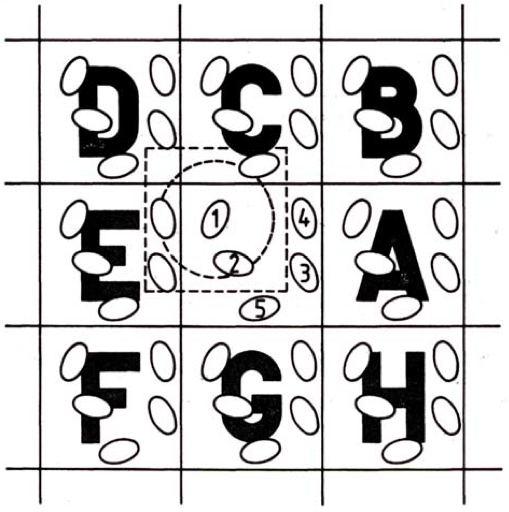
\includegraphics[width=.9\textwidth]{pics/ewald}
  \captionof{figure}{In the Ewald summation, the system is repeated  on each side of itself.}
  \label{fig:ewald}
\end{minipage}
\end{minipage}
\vspace{0.1cm}

\noindent
The resulting potential is thus the sum of all interactions with the particles in the cells, summed over the number of cells that we have
\begin{equation}
V= \frac{1}{2} \sum _{\vec{n}} {     \sum_{i,j}^N {z_i z_j \abs{\vec{r}_{i,j} + \vec{n}}^{-1}}    },
\label{eq:ewald}
\end{equation} 
excluding the summation for  $i=j$ in the case of $\vec{n} = 0$. The Ewald sum is only conditionally converging and converges very slowly. Since Ewald never touched a computer, the terms over which he intended to take the sum ($\vec{n}$) are of infinite number. What one has to do in reality is to truncate the sum at some point and try to estimate the error. Because of the nature of the algorithm, it is only used for few-particles systems. In \citet{dixon} there are several improvements that one can make in order to improve convergence. One possible technique consists of screening the charges out with a Gaussian distribution
$$
\rho_i\kl{r} = \frac{z_i \kappa^3}{\pi^{\frac{3}{2}}} \text{exp}\ekl{\kappa^2r^2}
$$ 
with some arbitrary smearing factor $\kappa$.
After having introduced the screening charges one has to cancel their total effect using charges of opposite sign.

\vspace{0.1cm}
\noindent
\begin{minipage}{\textwidth}
\begin{minipage}{.98\textwidth}
  \centering
  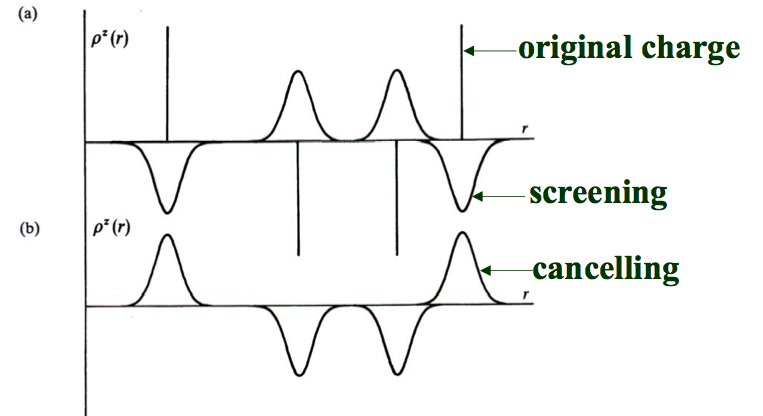
\includegraphics[width=0.85\textwidth]{pics/ewald_screening}
  \captionof{figure}{Screening of charges.}
  \label{fig:ewald_screening}
\end{minipage}
\end{minipage}
\vspace{0.1cm}

This way, the result is a very complicated sum that converges faster:
$$
V=\frac{1}{2} \sum_{i,j}   \kl  {   \sum_{\vec{n}} z_iz_j \frac {\text{erfc}\kl{\kappa \abs{\vec{r}_{i,j}+\vec{n}}}}{\abs{\vec{r}_{i,j} + \vec{n}}}  +  \frac{1}{\pi L^3} \sum_{\vec{k}\ne 0} z_iz_j \frac{4\pi^2}{k^2} \text{exp}\ekl{\frac{-k^2}{4\kappa^2}} \text{cos}\ekl{\vec{k}\vec{r}_{i,j}}    } -\frac{\kappa}{\sqrt{\pi}} \sum_i z^2_i
$$ with the \emph{error function} $\text{erfc}\kl{x} \equiv \frac{2}{\sqrt{\pi}} \int_x^\infty \text{exp}\ekl{-t^2}\text{dt}$. These formulaes are mentioned here only to show that the Ewald sum is a conceptually easy idea with a lot of implementation difficulties. It can be applied only under certain condition and we therefore break the discussion at this point.




\subsection{Particle Mesh Method}

\vspace{0.1cm}
\noindent
\begin{minipage}{\textwidth}
\begin{minipage}{.58\textwidth}
This method, invented by Eastwood and Hockney \citep{hockney,hockney_book}, is not very well suited for inhomogeneous distributions of particles. The concept is similar to what has been done in \citet{comp_phys} for solving the Poisson equation. We discretize the system using a mesh. In addition, we will now distribute the values of the density of masses confined in the cells on their vertices, in a way that is yet to be discussed. Through the discretized mass distribution we will be able to calculate the potential through \emph{Fast Fourier Transform} (FFT).
 \end{minipage}\hfill
\begin{minipage}{.38\textwidth}
  \centering
  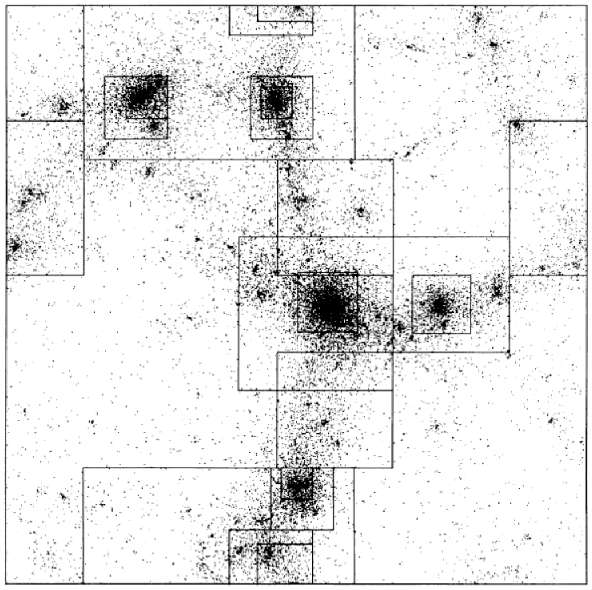
\includegraphics[width=\textwidth]{pics/particle_mesh}
  %\captionof{figure}{Comparison of the precision in the Verlet method and the predictor-corrector of various order.}
  \label{fig:particle_mesh}
\end{minipage}
\end{minipage}
\vspace{0.011cm}

\noindent
Once the potential is known, we can calculate the force exerted on the particles by interpolating the potential on the vertices. It is intuitive that the accuracy of the results depends on the following criteria:
\begin{itemize}
\item Errors should vanish for large distances between the particles.
\item Momentum should always be conserved (from $\vec{F}_{i,j}=-\vec{F}_{j,i}$).
\item Charges on the mesh and the interpolated forces should vary smoothly.
\end{itemize}
The method is not very efficient (unless one is able to adapt it) and time consuming for
\begin{itemize}
\item Inhomogeneous distribution of masses.
\item Strong correlations, like bound states in molecules.
\item Deviation from the point-like object approximation (e.g. tidal effects).
\item Complex geometries of the system.
\end{itemize} 
In these cases one might consider using the $P^3M$ or $AP^3M$ algorithms. These are presented later on in this chapter. Note that this method is very well behaved for gravitational interaction, which is in fact a force that is contributing even at large distances. Furthermore, gravitational interacting systems are characterized by overall low mass density (smooth variations in the potential) concentrated in pointlike coordinates more or less homogeneously distributed. That is indeed generally the case over very large regions of outer space. 

\subsubsection*{Implementation:}
Once we discretized our system we have more than one way to assign values at the vertices:

\begin{itemize}
\item Nearest Grid Point: consider the particle as on the nearest grid point.
\item Cloud in Cell: Distribute the total mass on the vertices of the cell proportionally to the inverse of the distance to the vertices.
\end{itemize}

In the case of CiC distribution of the charges one approach can be to assign the following density to the vertices of a cell containing a particle with coordinates $(x,y)$:

\begin{align*}
\rho_{i,j} &= q(x_{i+1}-x)(y_{i+1}-y) \\
\rho_{i+1,j} &= q(x-x_{i})(y_{i+1}-y) \\
\rho_{i,j+1} &= q(x_{i+1}-x)(y-y_{i}) \\
\rho_{i+1,j+1} &= q(x-x_{i})(y-y_{i}) 
\end{align*}
Note that the sum of the four vertices simply gives $q$.


From electrodynamics we know that the potential at a certain point $\vec{r}$ is given by the convolution of the density $\rho\kl{\vec{r}}$ and the green's function for the potential (e.g. $g\kl{\vec{r}}= \frac{G}{\abs{\kl{r}}}$ for the gravitational potential):

\begin{equation}
\phi\kl{\vec{r}} = \int \rho \kl{\vec{r}\,'}g\kl{\vec{r}-\vec{r}\,'}\text{d}\vec{r}\,'.
\end{equation}
In Fourier space this transforms to a simple multiplication, and there is no need of integration:

\begin{equation}
\tilde{\phi}\kl{\vec{k}} = \tilde{\rho} \kl{\vec{k}'}\tilde{g}\kl{\vec{k}-\vec{k}'}
\end{equation}
Having the the field at every point, one can calculate the force at every vertex of the mesh and then interpolate  the forces on the corners of the mesh to find the force that is exerted by the field on a particle.


As already mentioned, the PM algorithm is  not very well suited for inhomogeneous distributions of particles, strong correlations like bound states or complex geometries. In these cases one can use  the P$^3$M, the AP$^3$M, tree codes or multiple expansions. One important application of this can be found in astrophysics, where the spatial distribution of stars and galaxies is very heterogeneous. A very good reference for further reading is \citet{pfalzner}.

\subsubsection*{P\textsuperscript{3}M (Particle-Particle Particle Mesh):}

For particles with close neighbours we can decompose the force acting on it into two terms:
\begin{equation}
\vec{F} = \vec{F}_s + \vec{F}_l,
\end{equation}
where the first term denotes short distance interactions and the second term  long distance interactions. This approach has the drawback that the long-range potential field has to be computed for each particle, as the contributions to the potential field are not constant. We still have not solved the problem of heterogeneity, since most of the grid points are empty and this results in a big waste of computation time.

\subsubsection*{AP\textsuperscript{3}M (Adaptive Particle-Particle Particle Mesh):}

We will adapt the mesh to the particles density by using an adaptive mesh with fine resolution where particle density is higher. 

\vspace{0.1cm}
\noindent
\begin{minipage}{\textwidth}
\begin{minipage}{.58\textwidth}
As an example, one can refine a cell as long as there are more particles than a certain accepted quantity (see Fig. \ref{fig:quad_tree}). The book-keeping of these structures can be realized using trees that similar to the linked cell algorithms. The advantage of this method is that we are not tied anymore to a fixed geometry and that we can deal with inhomogeneous distributions. In these methods the most expensive part (from a computational point of view) is the Fourier transformation. There are a number of refinements that one can take and the computation of the FFT could cover an entire course on itself. Being a very important field of study, more information about the Fourier transformation can be easily found in literature and on-line (e.g. \citet{fourier}).
 \end{minipage}\hfill
\begin{minipage}{.4\textwidth}
  \centering
  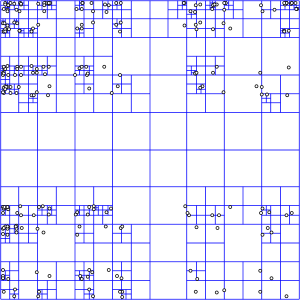
\includegraphics[width=\textwidth]{pics/quad_tree}
  \captionof{figure}{A mesh adapted to the local differences in particle density.}
  \label{fig:quad_tree}
\end{minipage}
\end{minipage}

\vspace{0.1cm}
The clusters can then be treated as \emph{quasi-particles}. They form hierarchical structures that can be organized into quad trees. The bookkeeping of the structures is still a very active field of research. The advance in the simulation of many-body systems often depends on the development of this technique. As to date, it is possible to simulate the interaction of $\propto 10^{11}$ stars.

\noindent
\begin{minipage}{\textwidth}
  \centering
  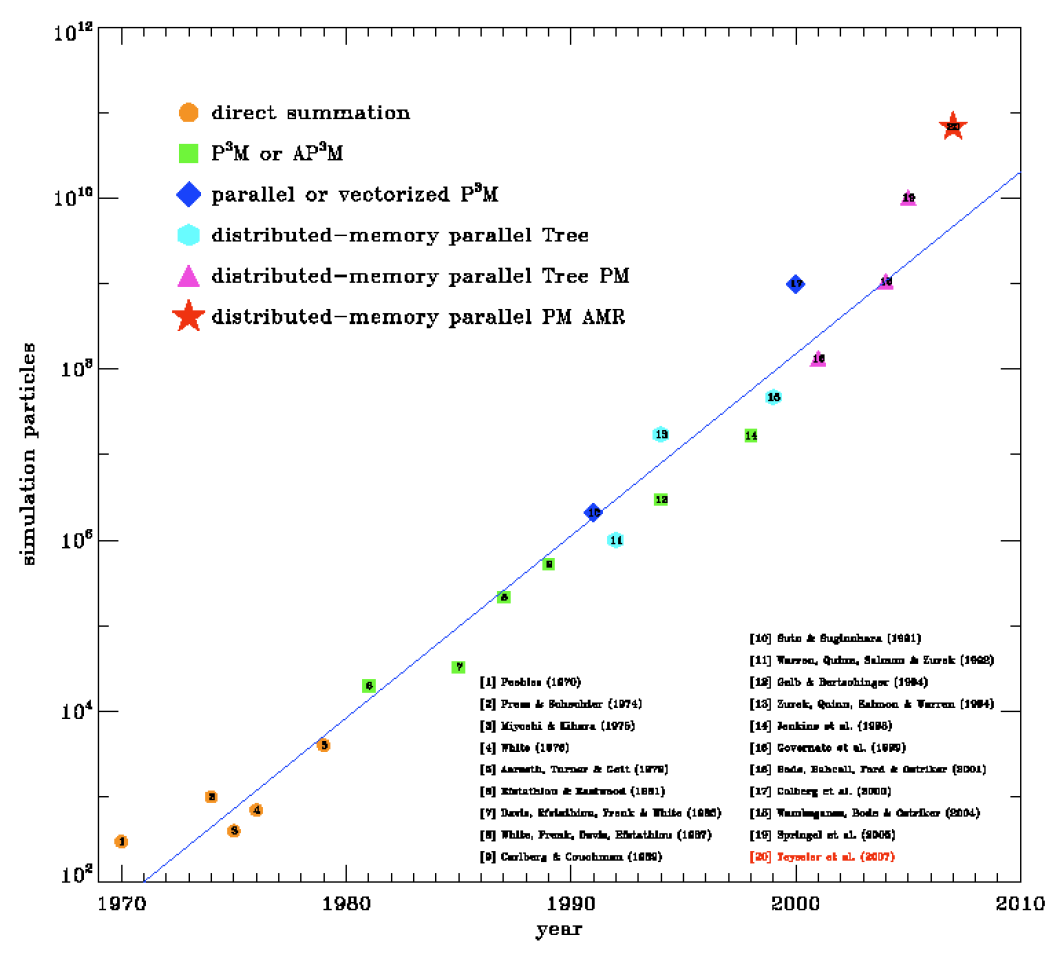
\includegraphics[width=.8\textwidth]{pics/stars}
  \captionof{figure}{Many-particle systems simulations in the last decades. Note that the number of simulated particles is scaled logarithmically. This is in accordance to the observation made by Gordon E. Moore in 1965. Moore noted that the quantity of processed information was doubled approximately every two years. For the interested reader, the considerations made by Amdahl and Gustafson regarding computation and parallelization are worth of a check.}
  \label{fig:stars}
\end{minipage}

\subsection{Reaction Field Method}
In the case of more complex interactions (e.g. composed molecules or non-point-like particles) a good solution is to ignore the complexity of distant particles and only take into account their mean effect while calculating explicitly the interaction with close particles. The concept finds its root in the work of Onsager in his work on the dielectric constant \citep{onsa_reaction} but it was introduced as an explicit computational technique in the 70s \citep{reaction1,reaction2}.

\vspace{0.1cm}
\noindent
\begin{minipage}{\textwidth}
\begin{minipage}{.5\textwidth}
This method is mostly used for the simulation of dipole-dipole interactions. We will consider the field of a cavity $N_i$ generated by the dipole moments $\vec{\mu}_j$ of the particles inside the cavity of radius $r_c$:
\begin{equation}
E_i = \frac{2(\epsilon_s-1)}{2(\epsilon_s+1)}\frac{1}{r^3_c}\sum_{j\in N_i}{\vec{\mu}_j}= \text{``reaction field''}
\end{equation}
and treat the effect of all the particles outside as if they where a homogeneous distribution of dielectricum. The resulting total force on the particle $i$ is then:
\vspace{0.2cm}
\begin{equation}
\vec{F}_i = \sum_{j\in N_i}{\vec{F}_{i,j}+E_i\times\mu_i}.
\end{equation}
\end{minipage}\hfill
\begin{minipage}{.45\textwidth}
  \centering
  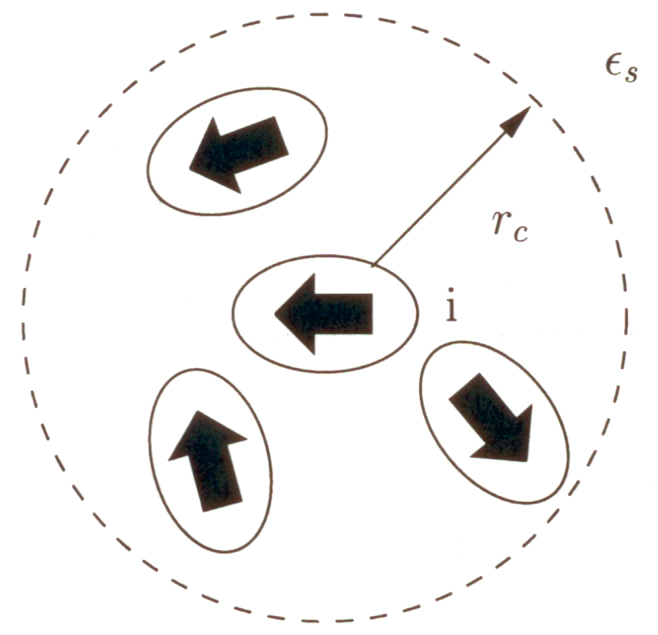
\includegraphics[width=\textwidth]{pics/reaction_field}
  \captionof{figure}{Only the interaction with particles nearby is considered. The rest of the system is summarized in a background field.}
  \label{fig:reaction_field}
\end{minipage}
\end{minipage}
\vspace{0.1cm}




\vspace{0.2cm}
\noindent
\begin{minipage}{\textwidth}
\begin{minipage}{.45\textwidth}
As the particles are moving, the number of particles inside the cavity will not remain constant. This will cause a jump in forces since the influence is weakened instantaneously. To avoid this effect one can introduce a weighting factor to the contribution of the particle that depends on its distance (see fig.\ref{fig:attenuation}).:
\begin{equation}
g(r_j)=\begin{cases}
  1,  & \text{for }r_j<r_t\\
  \frac{r_c-r_j}{r_c-r_t}, & \text{for }r_t \le r_j \le r_c \\
	0 , & \text{for }r_c < r_j
\end{cases}
\end{equation}

\end{minipage}\hfill
\begin{minipage}{.5\textwidth}
  \centering
  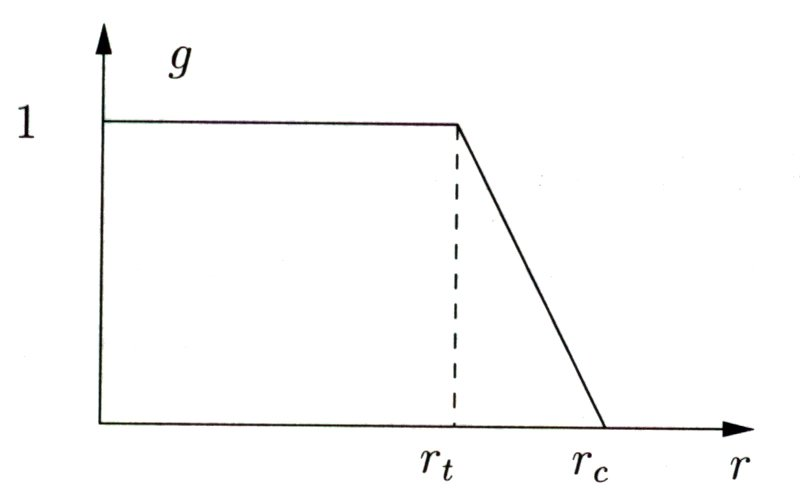
\includegraphics[width=\textwidth]{pics/attenuation}
  \captionof{figure}{Attenuation of the effects of a particle leaving/entering the cavity through linear interpolation.}
  \label{fig:attenuation}
\end{minipage}
\end{minipage}
\vspace{0.1cm}










